\documentclass{beamer}

\usetheme{simple}

\usepackage{scalerel,xparse}
\usepackage{lmodern}
\usepackage[scale=2]{ccicons}
\usepackage{ulem}
\usepackage{tikz}
\usetikzlibrary{positioning,calc,automata}
\usepackage{algorithm}
\usepackage{algorithmic}
\usepackage{caption}
\usepackage{listings}
\usepackage{xcolor}

% Watermark background (simple theme)
\setlength{\parindent}{0cm}
\setwatermark{
\includegraphics[height=8cm]{img/chungus_polar.png}}


\title{CSC363H5 Tutorial 5}
\subtitle{warning: do not attempt to learn social skills from me}
\date{\today}
\author{Paul ``sushi{\textunderscore}enjoyer'' Zhang}
\institute{University of Chungi (in polar coordinates)}

\NewDocumentCommand\emojisushi{}{
    
\includegraphics{img/1f363.png}
}
\NewDocumentCommand\emojimoyai{}{
    
\includegraphics{img/1f5ff.png}
}
\NewDocumentCommand\emojiflushed{}{
    
\includegraphics[scale=0.1]{img/flushed.png}
}

\begin{document}

\maketitle

\begin{frame}{Learning objectives this tutorial}
By the end of this tutorial, you should...
\begin{itemize}
\item Be able to come up with terrible CSC363 flirtatious quotes that are almost as bad as mine.
\item Be able to state what $A \leq_m B$\footnote{This is read ``$A$ is $m$-reducible to $B$''.} means. 
\item Understand why if $A \leq_m B$ and $A$ is c.e., then so is $B$.
\item Appreciate the fact that reading week is in 3 days, and then realize your assignment is also in 3 days ;-;\footnote{so ask me any questions you have!}
\end{itemize}
\end{frame}

\begin{frame}{Some readings (again, certified by \texttt{helo\textunderscore fish.jpg})}
\begin{itemize}
\item Chapter 7.1, 7.2 (up to page 107)
\item Chapter 10.1, 10.2, 10.3
\end{itemize}
Again, read those to cheat on the homework! honestly though, it would really help with the homework questions, and it contains a solution to at least one of the homework questions.
\begin{figure}[h]

\includegraphics[scale=0.3]{img/helo_fish_certified.jpg}
\end{figure}
\end{frame}

\begin{frame}{here's valentines day chungus \textless 3}
\begin{columns}
\column{0.4\linewidth}
\begin{figure}[h]
\centering

\includegraphics[scale=1]{img/chungus_wtf.jpg}

pls ignore watermarks.\\
because i'm low budget.
\end{figure}
\column{0.5\linewidth}
\begin{figure}[h]
\centering

\includegraphics[scale=1]{img/favorite_fish.jpg}
\end{figure}
\end{columns}
\end{frame}

\begin{frame}{DISCLAIMER}

{\color{red} DO NOT attempt to use any of the terrible pick-up lines you encounter in this tutorial, labelled in red. You have been warned.}\footnote{I do not make any copyright claims to any of these awkward flirting lines.}

Using these pick-up lines may result in:
\begin{itemize}
\item Being called to the principal's office.
\item Lovesickness, emotional pain, melancholy.
\item Severe social withdrawal and repulsion.
\item Prosecution via the \textit{Copyright Act} (or whatever copyright policy your jurisdiction has).
\item Forfeiture of privilege of eating sushi (or whatever your favourite food is). 
\item Music torture via the song ``Big Chungus''.
\end{itemize}
\end{frame}

\begin{frame}{Just a quick note for Q4 of the assignment!}
hopefully you have started the assignment already! D:

\vspace{2mm}

in Q4, by ``the set of partial computable functions is c.e.'', we mean the set
$\{e \in \mathbb N: \text{$\varphi_e$ is p.c.}\}$ is c.e.. By ``the set of (total) computable functions is not c.e.'', we mean the set $\{e \in \mathbb N: \text{$\varphi_e$ is total}\}$ is not c.e..

\vspace{2mm}

{\color{red} \textbf{Task:} prove that the set of good memories we will create is not computably enumerable. \emojiflushed}

\begin{figure}[h]
\centering

\includegraphics[scale=0.2]{img/helo_fish_unacceptable.jpg}
\end{figure}
\end{frame}

\begin{frame}{$m$-reduction? \emojiflushed}
Let $A, B \subseteq \mathbb N$ (as always!). We say $A \leq_m B$ (read ``$A$ is $m$-reducible to $B$'') if there exists a \textit{computable} function $f$ such that
$$x \in A \Leftrightarrow f(x) \in B.$$ 

Note: $f$ doesn't have to be a bijection! it doesn't even have to be injective.

\begin{figure}[h]
\centering
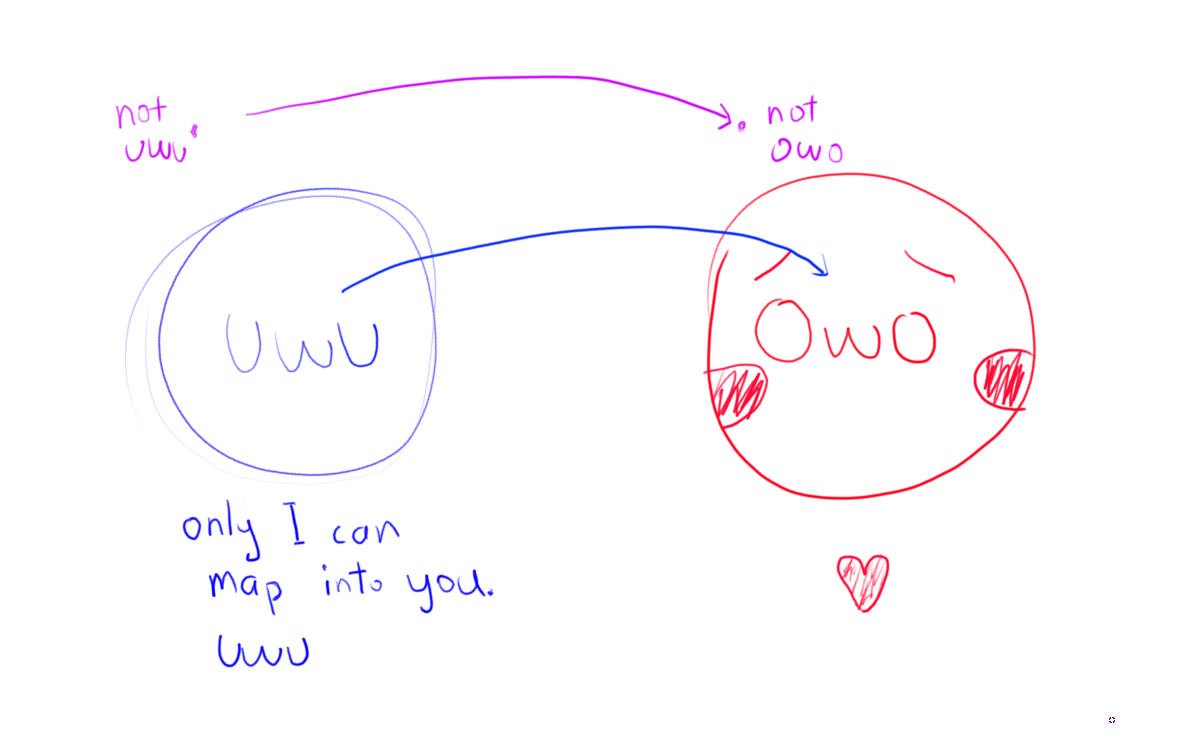
\includegraphics[scale=0.23]{img/uwu_owo.png}
\end{figure}

\end{frame}

\begin{frame}{$m$-reduction? \emojiflushed}
Let $A, B \subseteq \mathbb N$ (as always!). We say $A \leq_m B$ (read ``$A$ is $m$-reducible to $B$'') if there exists a \textit{computable} function $f$ such that
$$x \in A \Leftrightarrow f(x) \in B.$$ 

Example: if $A = \{0, 2, 4, \ldots\}$ and $B = \{0, 4, 8, \ldots\}$. Then $A \leq_m B$, since $f(x) = 2x$ is a computable function that satisfies $x \in A \Leftrightarrow f(x) \in B$.

\vspace{2mm}

Example: if $A$ is any computable set and $B = \{1\}$, then $A \leq_m B$ via $f(x) = I_A(x)$.

\end{frame}

\begin{frame}{$m$-reduction? \emojiflushed}

{\color{red} Are you a natural number? Cuz I am, and we can apply the Cantor pairing function \emojiflushed \emojisushi}

\begin{figure}[h]
\centering

\includegraphics[scale=0.2]{img/helo_fish_unacceptable.jpg}

Again, do not attempt to use these lines. I take no responsibility for any potential injuries you may incur from using these quotes.
\end{figure}

(either way, I hope you recall the Cantor pairing function!)

\end{frame}

\begin{frame}{$m$-reduction? \emojiflushed}

\textbf{Task:} Let $K_0 = \{\langle x, y \rangle: \varphi_x(y) \downarrow\}$. Show that $K \leq_m K_0$ by finding a computable function $f$ such that $x \in K \Leftrightarrow f(x) \in K_0$.\footnote{$K = \{x: \varphi_x(x) \downarrow\}$.}

\vspace{2mm}

{\color{red} \textbf{Task:} Show that I am $m$-reducible to you. Conclude that there exists a computable function $f$ that maps me to you exclusively. \textless 3}

\vspace{2mm}

{\color{red} \textbf{Task:} Show that my feelings for you are in $\overline{K}$. }

\begin{figure}[h]
\centering

\includegraphics[scale=0.3]{img/free_smiley.jpg}

cursed smiley.
\end{figure}

\end{frame}

\begin{frame}{$m$-reduction? \emojiflushed}

\textbf{Task:} Let $K_0 = \{\langle x, y \rangle: \varphi_x(y) \downarrow\}$. Show that $K \leq_m K_0$ by finding a computable function $f$ such that $x \in K \Leftrightarrow f(x) \in K_0$.\footnote{$K = \{x: \varphi_x(x) \downarrow\}$.}

\vspace{2mm}

Answer: let $f(x) = \langle x, x \rangle$. Then
$$x \in K \Leftrightarrow \varphi_x(x) \downarrow \Leftrightarrow \langle x, x \rangle \in K_0.$$

\end{frame}

\begin{frame}{$m$-reduction? \emojiflushed}

The following theorem is saying that if $A \leq_m B$, then $B$ is ``at least as hard to compute as $A$'', in some sense. 

\begin{theorem}
\begin{enumerate}
\item If $A \leq_m B$ and $B$ is computable, then $A$ is computable. 
\item If $A \leq_m B$ and $B$ is c.e., then $A$ is c.e..
\end{enumerate}
\end{theorem}


\textbf{Task:} Prove the above.

Hint: \begin{enumerate}
\item Show that we can decide whether something is in $A$ or not.
\item Using the normal form theorem, we can suppose there exists a computable relation $R$ such that
$$x \in B \Leftrightarrow \exists y \, R(x, y).$$
Show that $A \in \Sigma^0_1$.
\end{enumerate}

\end{frame}

\begin{frame}{$m$-reduction? \emojiflushed}
\begin{theorem}
\begin{enumerate}
\item If $A \leq_m B$ and $B$ is computable, then $A$ is computable. 
\item If $A \leq_m B$ and $B$ is c.e., then $A$ is c.e..
\end{enumerate}
\end{theorem}

\textit{Proof}: 
\begin{enumerate}
\item Let $f$ be a computable function so that $x \in A \Leftrightarrow f(x) \in B$. Then to check whether some arbitrary $x \in A$, we just check whether $f(x) \in B$ or not. 
\item Let $f$ be a computable function so that $x \in A \Leftrightarrow f(x) \in B$. Using the normal form theorem, we can suppose there exists a computable relation $R$ such that
$$x \in B \Leftrightarrow \exists y \, R(x, y).$$
Then
$$x \in A \Leftrightarrow f(x) \in B \Leftrightarrow \exists y \, R(f(x), y).$$
\end{enumerate}

\end{frame}

\begin{frame}{\textless 3}
\begin{theorem}
\color{red}
If your feelings are so much harder to compute than my feelings, then\\ I \textless 3 you.
\end{theorem}

\begin{figure}[h]
\centering

\includegraphics[scale=0.3]{img/chubbyemu.png}
\end{figure}

\end{frame}

\begin{frame}{Exercise 7.1.6}
Again, $K_0 = \{\langle x, y \rangle: \varphi_x(y) \downarrow\}$.
\vspace{2mm}

\textbf{Task:} Convince yourself that $K_0$ is c.e..

\vspace{2mm}

\textbf{Task:} Let $A \subseteq \mathbb N$. Show that $A$ is c.e. if and only if $A \leq_m K_0$. 

\vspace{2mm}

Hint: Normal form theorem! $A$ is c.e. implies $A = W_e$ for some $e$. 

\vspace{2mm}

\pause
Answer: Suppose $A$ is c.e.. Then $A = W_e$ for some $e$. Consider the function $f(x) = \langle e, x\rangle$: 
$$x \in A \Leftrightarrow x \in W_e \Leftrightarrow \varphi_e(x) \downarrow \Leftrightarrow \langle e, x \rangle \in K_0.$$
Conversely suppose $A \leq_m K_0$. Since $K_0$ is c.e., by the theorem we have proven, $A$ is also c.e..

\end{frame}

\begin{frame}{363 is hard ;-;}

{\color{red} are you CSC363? because i don't want to fail you ;-;}

\vspace{2mm}

{\color{blue} are you a math course? i'm sorry, i'd prefer passing on you. :(}

\vspace{2mm}

\begin{figure}[h]
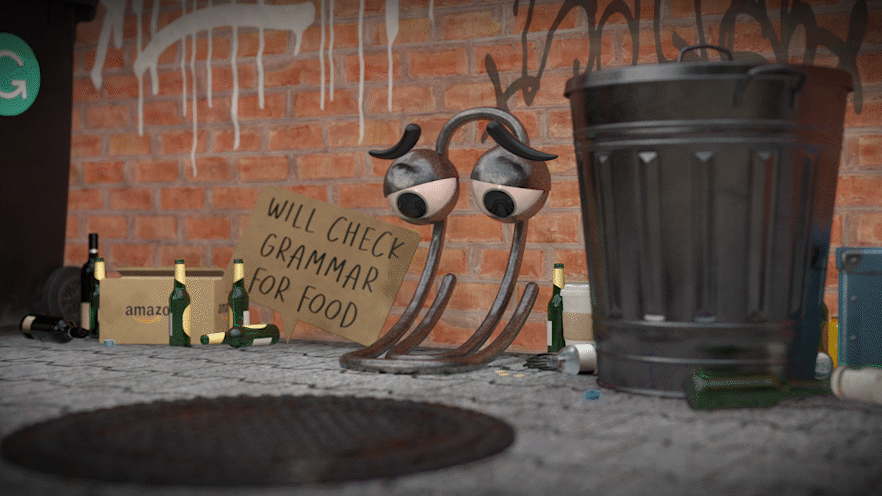
\includegraphics[scale=0.35]{img/grammar.png}
\end{figure}

\end{frame}

\begin{frame}{as you can see, you shouldn't ask me for relationship advice.}
i planned the tutorial to end here, i don't have any more content prepared. sorry ;-; and have a nice day! here's some plain sushi

\begin{figure}[h]
\centering

\includegraphics[scale=0.2]{img/plain_sushi.jpg}
\end{figure}

\vspace{4mm}

{\color{red} \textbf{Task:} come up with pickup lines that are nearly as bad as mine.}

\vspace{2mm}

{\color{red} \textbf{Task:} convince yourself that instead of $m$-reducibility, you've learned more about how to convince people to stay away from you.}

\end{frame}













\end{document}